\chapter{Framework EACirc}
\label{chap:eacirc}

Testovanie náhodnosti štatistickými testami má však aj svoje nevýhody. Pre zjednodušenie si predstavme, že sa v batérii nachádza iba jeden test, ktorý testuje, či je počet núl a jednotiek približne rovnaký. Potom nie je zložité vytvoriť sekvenciu, ktorá testom prejde, napríklad postupnosť, v ktorej sa pravidelne striedajú nuly a jednotky. Avšak pravdepodobnosť, že by takáto sekvencia bola výstupom z naozaj náhodného generátora je veľmi malá. Nevýhodou štatistických sád je to, že obsiahnuté testy dokážu odhaliť iba nezrovnalosti, na ktoré boli naprogramované. Preto sa v štatistických sadách nachádza veľké množstvo testov, avšak každý test pridáva iba jednu vlastnosť, ktorú kontroluje. Ale náhodnosť neznamená spĺňať presne danú množinu vlastností. Z toho vyplýva, že výsledok zo štatistických testov nemusí vždy garantovať, že sú dáta naozaj náhodné, respektíve nenáhodné. Tento nedostatok rieši alternatívny prístup, \textit{Framework EACirc}~\parencite{eacirc-github}. 

Prístup EACircu je oproti štatistickým testom úplne odlišný. Vo svojej podstate je to nástroj, ktorému nastavíte dva prúdy dát a on hľadá medzi nimi rozdiel. Toto vykonáva prostredníctvom vytvárania funkcie, ktorá dokáže určiť, či dostala dáta z prvého, respektíve druhého prúdu. Následne je na základe nájdenia, respektíve nenájdenia takejto funkcie určená podobnosť týchto dvoch prúdov. Ak chceme aby EACirc fungoval podobne ako štatistické testy, teda aby určoval aká je pravdepodobnosť, že sú preverované dáta náhodné, stačí nastaviť ako jeden z prúdov dát naozaj náhodné dáta. V prípade, že EACirc nenájde rozdiel medzi náhodnými dátami a preverovanými dátami znamená to, že sú tieto dáta pravdepodobne tiež náhodné. Naopak, ak sa rozdiel nájde, znamená to, že tieto dáta pravdepodobne nie sú náhodné. Z toho vyplýva, že pre korektné fungovanie EACircu je veľmi dôležité použiť kvalitné náhodné dáta. V opačnom prípade EACirc nebude vedieť ako majú naozaj náhodné dáta vyzerať a preto môže označiť za náhodné aj dáta, ktoré síce nebudú náhodné, ale budú podobné dátam, o ktorých si EACirc myslí, že náhodné sú. Inými slovami by sa dalo povedať, že EACirc dokáže byť v určovaní náhodnosti len taký dobrý, ako dobré su náhodné dáta, ktoré používa.

Častou požiadavkou na EACirc je to, aby fungoval podobne ako štatistické sady, teda aby rozlišoval medzi náhodnými dátami a dátami pochádzajúcimi zo šifrovacej respektíve hašovacej funkcie. Preto EACirc obsahuje integrované kryptografické funkcie, ktoré sa dajú jednoducho nastaviť ako jeden z prúdov. Jedná sa napríklad o kandidátov na funkciu SHA3~\cite{thesis-dubovec}, kandidátov na funkciu eSTREAM~\parencite{thesis-pristak} alebo tiež kandidátov zo súťaže CAESAR~\cite{ukrop-master}. Výsledky obsahujúce aj porovnanie so štatistickými testami pre funkcie zo súťaží SHA3 a eSTREAM, sú k dispozícii v nasledujúcich publikáciách~\parencite{ukrop-bc, svenda2013, svenda2014}.

\section{Princíp fungovania}
\label{sec:principle}

Vytváranie hore zmienenej funkcie pripomína pomyselnú skladačku. Zatiaľ čo štatistické testy sa dajú prirovnať k hotovej skladačke, s ktorou sa nedá hýbať, EACirc obsahuje iba samotné komponenty, z ktorých sa dá výsledná skladačka poskladať akýmkoľvek spôsobom. Najdôležitejšou úlohou EACircu je zložiť tieto komponenty do jedného celku tak, aby výsledná skladačka spĺňala požadované vlastnosti, teda aby funkcia opísaná touto skladačkou vedela rozlišovať medzi náhodnými dátami a skúmanými dátami. Na poskladanie používa samovzdelávací genetický algoritmus (detailný pohľad v \hyperref[sec:genetics]{sekcii 2.3}), ktorý najprv náhodne poskladá ľubovoľné kocky na seba a potom sa skladačku snaží malými zmenami vylepšovať.

Cieľom EACircu je využiť tento prístup na to, aby ním z jednoduchých operácií (vysvetlenie operácií v \hyperref[sec:nodes]{sekcii 2.2}) vytvoril funkciu, ktorá bude vykonávať postupnosť týchto operácií a dokáže zo vstupu zistiť, či dostala náhodné dáta alebo preverované dáta. S týmto prístupom sa spája niekoľko výhod, napríklad:
\begin{myItemize}
	\item \textbf{Na vytváranie testov nie je potrebná žiadna ľudská aktivita}\\Testy zo štatistických sád bývajú založené na matematických problémoch, nad ktorými museli ľudia stráviť množstvo času.
	\item \textbf{Testovanie aj zatiaľ nepoznaných problémov}\\Štatistické sady neobsahujú testy na všetky vlastnosti nenáhodných dát, na druhej strane EACirc vytvára hľadanú funkciu náhodne, z toho vyplýva, že v nej môže teoreticky testovať čokoľvek, k čomu genetický algoritmus dospeje.
\end{myItemize}

\section{Vysvetlenie funkcie na rozlišovanie prúdov}
\label{sec:nodes}

Celá skladačka je v skutočnosti graf. Každá kocka tejto skladačky reprezentuje jeden uzol a spojenie dvoch kociek znamená, že medzi týmito uzlami vedie cesta. Tento graf je zoskupený do horizontálnych vrstiev, ktoré sú poskladané na seba. V každej vrstve sa nachádza niekoľko uzlov. Cesty vedú len smerom zhora nadol a to len medzi vrstvami idúcimi bezprostredne za sebou tak, ako to je vidieť na \hyperref[obr:circuit-example]{obrázku 2.1}. Prvá vrstva je vstupná a posledná výstupná. V ďalších odsekoch si vysvetlíme princíp fungovania grafov, ktoré budeme nazývať aj obvody. Teda akým spôsobom dokáže jednoduchý graf určiť, či dostal dáta z prvého, respektíve druhého prúdu. 

\begin{figure}[h!]
	\centering
	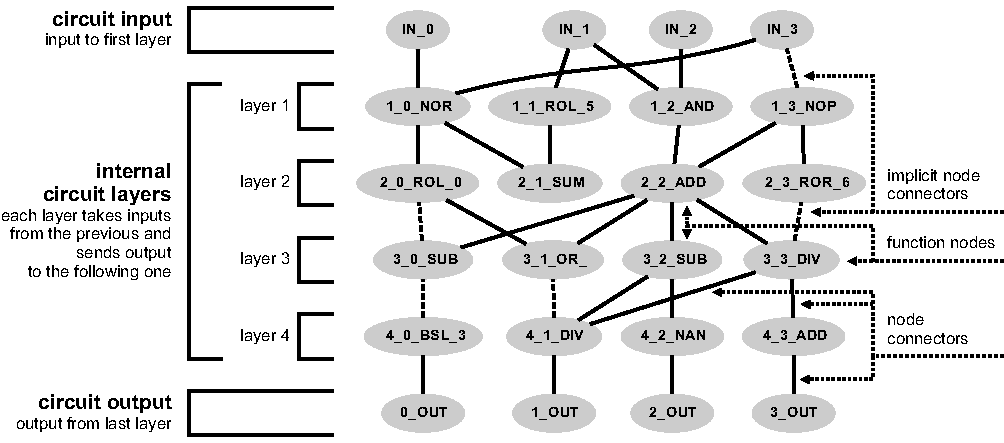
\includegraphics[scale=0.8]{./img/circuit-final.pdf}
	\caption{Vizualizácia obvodu z {bakalárskej práce}~\parencite{ukrop-bc} Martina Ukropa.}
	\label{obr:circuit-example}
\end{figure} 

Každý uzol v sebe nesie uloženú informáciu. Na tomto mieste je okrem iného uložené aj to, akú funkciu bude tento uzol vykonávať. Každý z uzlov môže vykonávať práve jednu z nasledujúcich funkcií:
\begin{myItemize}
	\item \textbf{Bitové operátory}\\AND, OR, XOR, NOR, NAND, ROTL, ROTR, BITSELECTOR
	\item \textbf{Aritmetické funkcie}\\SUM, SUBS, ADD, MULT, DIV
	\item \textbf{Operátor identity}\\NOP
	\item \textbf{Operátor na priame čítanie zo vstupu}\\READX
\end{myItemize}
Uzol v sebe ďalej môže obsahovať aj parametre, ktoré niektoré funkcie potrebujú na ich vykonanie. Celkový limit na uložené dáta v rámci jedného uzlu je 4B.

Vykonávanie funkcie v rámci jedného uzla prebieha nasledovne. Na začiatku uzol dostane niekoľko vstupov z predchádzajúcej vrstvy. Všetky tieto vstupy spracuje na základe funkcie, ktorú ma vykonávať, napríklad vykoná medzi všetkými vstupmi operáciu \textit{AND}. Konečný výsledok posiela uzlom v nasledujúcej vrstve ako vstup. Voľba od koho uzol dostane dáta a kam ich po vykonaní pošle prebieha náhodne. Preto môže nastať aj situácia, kedy nemá uzol žiadne vstupy ani výstupy, to znamená, že takýto uzol vôbec neovplyvňuje konečný výsledok. Prvá vrstva je vstupná, čiže na vstupe dostane dáta priamo z niektorého z prúdov. Následne dáta prebublávajú smerom nadol tak, že každý uzol z dátami vykoná funkciu, ktorú ma v sebe uloženú a výsledok pošle o úroveň nižšie. Posledná vrstva je výstupná, to znamená, že z dát ktoré sú výstupom z poslednej vrstvy sa zisťuje, či dáta pochádzajú z prvého, alebo druhého prúdu.

Použitie jednoduchých funkcií môže v konečnom dôsledku vyústiť do zložitejších konštrukcií. Dokonca sa môže docieliť podobného testu ako sa vyskytuje v štatistických sadách. Avšak použitie genetického algoritmu prináša aj možnosť vymyslieť lepšie a silnejšie testy ako sa nachádzajú v batériách. Preto je našim úmyslom vytvoriť pre genetiku čo najlepšiu situáciu na skonštruovanie výsledného obvodu. Následkom je myšlienka, nepoužívať v~uzloch iba jednoduché funkcie (napríklad AND, OR atď.), ale vykonávať v uzloch niečo zložitejšie, napríklad inštrukcie pochádzajúce z kódu, ktorý vygeneroval testovaný prúd dát. V \hyperref[chap:eacirc-jvmsim]{kapitole 3.} si tieto uzly bližšie predstavíme.


\section{Genetika}
\label{sec:genetics}

V tejto sekcii si objasníme prečo sa algoritmus používaný na vytváranie najlepšieho obvodu nazýva genetický. Ďalej si preberieme aj to, ako sa postupne z obyčajného náhodného grafu, ktorý nemá najlepšiu úspešnosť v rozlišovaní toho, z ktorého prúdu dostal na vstupe dáta, vytvorí graf, ktorý má spomenutú úspešnosť vyššiu.

{Genetické programovanie}~\cite{koza1992genetic} vzniklo za účelom naučiť počítače riešiť rôzne problémy bez toho, aby na to boli explicitne naprogramované. Teda aby počítače vedeli riešiť problémy bez toho, aby im bolo povedané ako presne to urobiť. V skutočnosti sa jedná o~algoritmy výsledkom ktorých je štruktúra, ktorá nejakým spôsobom reprezentuje počítačový program. V prípade EACircu je touto štruktúrou graf. Keďže sa jedná o~genetický algoritmus, tento graf označujeme okrem pojmu obvod aj jedinec. 

Algoritmus sa volá genetický aj preto, lebo jeho priebeh pripomína fungovanie genetiky v prírode. Priebeh algoritmu sa delí na tzv. generácie. V každej generácií existuje niekoľko jedincov. Každý jedinec je reprezentovaný grafom a cieľom je postupne tieto grafy vylepšovať tak, aby v každej nasledujúcej generácii boli úspešnejší jedinci v riešení zadaného problému, v našom prípade v riešení problému náhodnosti. Vytváraním nových generácií sa docieľuje toho, že sa jedinci postupne učia ako riešiť zadaný problém, preto sa tento algoritmus nazýva aj samovzdelávací~\cite{machine_learning}. Celý priebeh algoritmu sa dá opísať nasledujúcimi krokmi:\vspace{-10pt}
\begin{enumerate}
	\item \textbf{Náhodné vygenerovanie jedincov}\\Vytvorí sa tzv. iniciálna populácia jedincov. Tieto jedince sa tvoria náhodne, to znamená, že sa bude jednať o niekoľko grafov, kde každý bude vytvorený náhodne.
	\item \textbf{Určenie úspešnosti}\\Úspešnosť sa vypočíta pomocou tzv. funkcie vhodnosti, ktorá je pre správny priebeh veľmi dôležitá. Každý z jedincov bude mať nejakú úspešnosť, niektorí ju budú mať lepšiu a niektorí horšiu.
	\item \textbf{Vyradenie neúspešných obvodov}\\Keďže potrebujeme aby nasledujúca generácia bola čo najlepšia, musíme ju založiť len na tých najlepších jedincoch, slabšie jedince preto vyradíme.
	\item \textbf{Skríženie najúspešnejších jedincov}\\Skrížením dostaneme novú populáciu jedincov. Cieľom kríženia je dosiahnuť novú silnejšiu generáciu.
	\item \textbf{Náhodná mutácia niektorých jedincov}\\Aby sa zabránilo zaseknutiu v lokálnom maxime, je potrebné urobiť náhodnú mutáciu, napríklad odobrať niektorú z ciest, alebo zmeniť niektorý z uzlov. Mutácia prebieha tak, že sa postupne prechádza grafom a pri každom uzle, respektíve hrane sa z nejakou pravdepodobnosťou vykoná mutácia.
	\item Kroky 2-5 su prevádzané v cykle až kým sa nedosiahne požadovaná úspešnosť alebo kým sa nevyčerpá určený počet generácií.
\end{enumerate}
Úspešnosť jedinca sa zistí veľmi jednoducho. Z prúdov dát sa získa niekoľko vzoriek, ktoré sa nazývajú testovacie vektory. Dĺžka testovacieho vektora sa dá zvoliť pre každý beh osobitne. Pri experimentoch v tejto práci som obvykle používal dĺžku 16B a počet vektorov 1000 z~každého prúdu. Následne sa každému jedincovi predajú postupne všetky testovacie vektory a zistí sa s akou pravdepodobnosťou jedinec označil správne, či vektor pochádzal z prvého, respektíve druhého prúdu. 

Po skončení sa zistí, či je výstupom jedinec, ktorý naozaj dokáže rozlíšiť, či sa jedná o~dáta z prvého alebo druhého prúdu. Následne EACirc vyhlasuje, či sa jedná o~náhodné dáta. Toto vyhlásenie je však relevantné len v prípade, že je jedným z prúdov prúd náhodných dát. 

Generovanie náhodných hodnôt počas celého algoritmu sa vykonáva pomocou pseudo náhodného generátora. V žiadnom prípade sa však tento generátor nepoužíva na vytváranie prúdu, ktorý sa používa na porovnávanie s preverovanými dátami, jedná sa len o hodnoty, ktoré sa používajú pri vytváraní obvodov. V každom behu sa na začiatku zvolí náhodné počiatočné semienko a na ňom závisia všetky ďalšie vygenerované hodnoty. Takáto verzia generátora bola zvolená kvôli reprodukovateľnosti výpočtov. To znamená, kvôli tomu aby EACirc vracal rovnaké výsledky pre behy, ktoré majú rovnaké nastavenia a počiatočné semienko.

Na nastavenie všetkých hodnôt sa používa konfiguračný súbor, ktorý musí byť špecifikovaný pre každý beh. V rámci konfiguračného súboru sa nastavuje napríklad počet generácií, dĺžka testovacích vektorov alebo ich počet. Takisto sa v ňom volia prúdy, medzi ktorými sa bude v rámci behu rozlišovať. Príklad konfiguračného súboru je v prílohe.

\section{Interpretácia výsledkov}
\label{sec:result-interpretation}

EACirc má pre každý beh hypotézu, či sú skúmané dáta náhodné alebo nie. Na konci behu sa táto hypotéza buď potvrdzuje alebo zamieta. Ak sa hypotéza potvrdí, znamená to, že dáta sú náhodné, ak nie, tak EACirc našiel obvod, ktorý vie rozlíšiť medzi preverovanými a náhodnými dátami. To, či sa hypotéza zamietne alebo potvrdí sa rozhoduje podľa p-hodnoty, čo je hodnota, ktorá je výsledkom každého behu, a hladiny významnosti, čo je hodnota špecifikovaná v konfiguračnom súbore a určuje, ktorá je najväčšia hodnota, pre ktorú sa hypotéza ešte zamieta. To znamená, že po dokončení výpočtu sa získaná p-hodnota porovná s hladinou významnosti. Ak je p-hodnota menšia, hypotéza sa zamieta, inak sa potvrdzuje. 

Keďže sa počas celého priebehu algoritmu volia všetky hodnoty náhodne a nie vždy sa musí genetike podariť zostrojiť úspešný obvod, existuje istá pravdepodobnosť, takisto ako pri štatistických testoch, že EACirc aj náhodné dáta označí za nenáhodné a naopak. Preto sa výpočty vždy počítajú na viac behov, vždy s náhodným semienkom. Výsledok takýchto výpočtov bude pomer pre nás úspešných behov ku všetkým behom, teda percentuálne zastúpenie takýchto behov. Pre nás úspešné behy sú také, v ktorých bol EACirc úspešný v~hľadaní obvodu, to znamená v ktorých bola hypotéza zamietnutá. Ak je pomer menší ako hladina významnosti, väčšinou 5\%, znamená to, že EACirc bol úspešný v hľadaní obvodu len vo veľmi málo prípadoch a teda skúmané dáta sú náhodné. Čím vyšší pomer, tým vo viac behoch bol EACirc úspešný v~hľadaní obvodu a teda tým väčšia pravdepodobnosť, že dáta nie sú náhodné. Keďže sa spúšťa veľké množstvo behov EACircu naraz a v prípade veľkého množstva generácií spotrebuje jeden beh EACircu veľa času, bola do EACircu pridaná aj podpora zrýchlenia pomocou {nVidia CUDA technológie}~\parencite{novotny-bc}.



